\section*{Scénario}

L'étude de scénario a été une étape importante dans notre réflexion d'optimisation de l'ordonnanceur. Cette démarche nous a permis de lever situations et cas particuliers pour la conception de notre solution.
\\

Pour simplifier, dans la suite du rapport nous considérons être sur un monoprocesseur et les tâches bloquées par le verrou sont des threads.
\\

Considérons deux tâches : un éditeur de texte (A) et un compilateur (B). La 
tâche A détient un verrou et est moins prioritaire que B. La tâche A bloque 
plusieurs autres tâches dans son exécution, elle est donc la cible de notre 
optimisation : il faut trouver un moyen de favoriser A lors des élections pour 
débloquer plus rapidement les autres tâches endormies.

Une première solution, trop naïve, était de modifier la priorité de A afin 
d'assurer sa réélection. Dans les faits, cela aurait été de modifier le 
\verb|vruntime| de l'entité correspondante afin de la placer à gauche du 
\verb|rbtree|. Comme expliqué précédemment, cela pose plusieurs problèmes, 
notamment une modification risquée du scheduler mais aussi, est-ce vraiment la 
finalité attendue ?

En forçant le placement de la tâche à gauche de l'arbre on s'assure sans 
conteste une élection au prochain tour. Cependant cela implique que la tâche 
A passe devant toutes les autres tâches, y compris la tâche B, qui est plus 
prioritaire. Cette solution écrase donc toute la logique du système de priorité 
mise en place dans le scheduler. Ce constat nous a permis d'y voir plus clair, 
nous devons trouver une solution qui garde la hiérarchie des priorités : 
favoriser A ne doit pas être un inconvénient pour B.

Une réponse à ce problème peut être d'influencer sur la priorité d'origine 
attribuée à la tâche A. Par exemple, A s'exécute avec une priorité de 120 
(valeur par défaut) et B avec une priorité de 100. On peut très bien envisager 
d'augmenter la priorité de A pour la rendre plus prioritaire sans dépasser B. 
Augmenter la priorité de 10 semble être un bon choix, A aura donc une priorité 
de 110. Cependant, dans cet exemple l'intérêt est limité, cela devient plus 
intéressant si l'on ajoute une nouvelle tâche C, de priorité 120. Les tâches A 
et C commenceront donc avec la même priorité, mais A verra sa priorité augmenter
rapidement lorsque des tâches se bloqueront sur le verrou qu'elle détient. 
Ainsi, la tâche A sera favorisée face à des tâches de priorité équivalentes mais
ne sera pas un inconvénient pour les autres tâches.

Considérons maintenant que la tâche C est semblable à la tâche A, soit un autre éditeur de texte qui bloquera elle aussi des tâches par la prise d'un verrou. Les deux tâches se verront donc voir chacune augmenter leur priorité de 10. Cependant, par la prise de son verrou, A peut peut-être bloquer plus de tâche que C, mais du point de vue du scheduler A et C sont sur un pied d'égalité en matière de priorité. De ce constat est né l'idée d'influencer la priorité de la tâche en fonction du nombre de tâches bloquées par son verrou. 
\\

On introduit donc un système de \textbf{charge}, plus une tâche a une charge élevée, plus sa priorité évolue. La priorité d'une tâche sera augmentée dans un intervalle de 0 à 10 en fonction de sa charge. Reste à établir comment calculer la charge d'une tâche. 

Une première idée aurait été de calculer cette charge avec un système de pourcentage. Un compteur qui, au fur et à mesure de la vie d'exécution de la tâche A, compterait le nombre total de tâche qui peut potentiellement se bloquer sur le verrou. Un deuxième compteur, indiquant le nombre de tâches actuellement bloquées, permettrait de calculer un pourcentage de charge. Une simple division par 10 de la charge aurait permis de calculer l'augmentation de la priorité. Mais cette solution pose le problème de garder un compteur fiable sur le nombre de tâches pouvant potentiellement se bloquer sur le verrou. De plus le pourcentage de charge n'est pas très parlant. Imaginons que A et C ont toutes les deux une charge de 100\% mais A bloque 100 tâches contre 10 pour C. Bien que A devrait être plus favorisé il n'en reste que A et C auront toutes les deux une priorité augmentée de 10.
\\

Plutôt que de se perdre dans de lourds calculs de charge avec des pourcentages, nous avons décidé de s'orienter vers une implémentation plus simple. La charge correspondra au nombre total de tâches couramment bloquées sur le verrou. Ainsi, la priorité ajoutée à la tâche propriétaire du verrou restera toujours dans un intervalle de 0 à 10 mais fonctionnera par paliers : sur des échelons restant encore à définir, on peut envisager que toutes les 5 tâches bloquées la priorité se voit augmenter de 1, plafonnant ainsi l'augmentation à 50 tâches bloquées.
\\

Pour rendre cette implémentation plus efficace nous ajoutons le
mécanisme d'héritage de priorité. Considérons pour simplifier deux fils d'exécution
(tâche 1 et 3) qui partagent le même espace d'adressage et qui veulent accéder à une même section critique, et un processus (tâche 2) qui contient un seul fil d'exécution indépendant des deux 
premiers, dont les priorités sont définies comme ceci: Pri(3) $>$ Pri(2) $>$ 
Pri(1), même en considérant l'augmentation de priorité définie précédemment.
\\

NB: cette configuration peut être aussi atteignable avec 3 processus dont deux 
utilisent un segment de mémoire partagé ou bien 3 threads d'un même processus.
\\

Si la tâche 1, qui se trouve être la moins prioritaire, prend un futex et que 
la tâche 3, qui est la plus prioritaire, veut aussi l'acquérir, elle
devra se bloquer en attendant que la tache 1 libère le verrou. Étant donné que la tâche 2 possède une priorité plus élevée que le propriétaire du futex, elle sera choisie plus fréquemment par le scheduler. Ce comportement va ralentir l'exécution de la tâche 3, la plus prioritaire, qui est bloquée en attente de la libération du futex par la tâche 1.

\begin{figure}[h!]
	\centering
	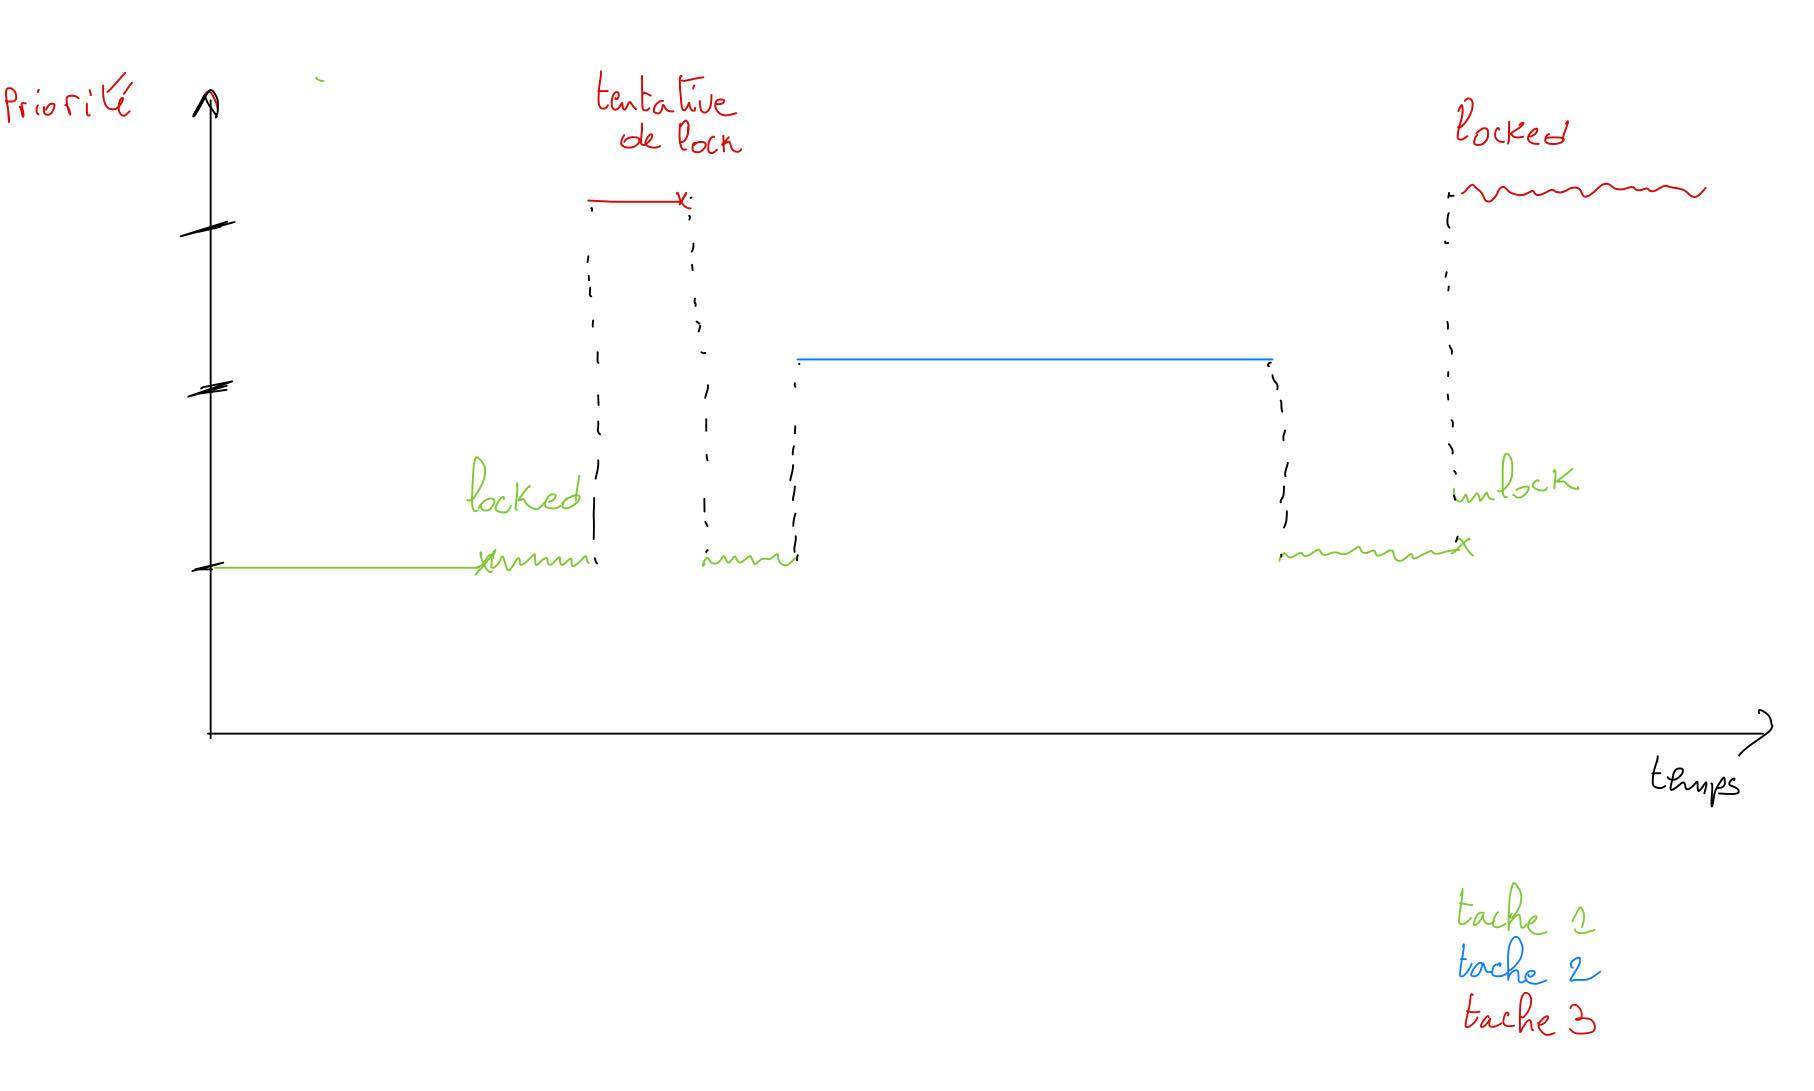
\includegraphics[scale=0.21]{include/without_inherit.jpg}
	\caption{Avancement des processus sans l'heritage de priorité}
	\label{fig:without_inherit}
\end{figure}

\newpage


L'idée ici est de modifier la priorité de la tâche 1 pour qu'elle soit plus 
prioritaire que la tâche 2. On peut atteindre cela en héritant de la 
priorité de la tâche 3, qui est plus prioritaire que la tâche 2. 

Ainsi, le propriétaire du verrou se verra attribuer, au cours de son exécution, la priorité de la tâche la plus prioritaire parmi toutes les tâches bloquées sur le verrou. De plus, l'augmentation de la priorité par rapport à la charge introduite précédemment sera appliquée à cette nouvelle priorité.

\begin{figure}[h!]
	\centering
	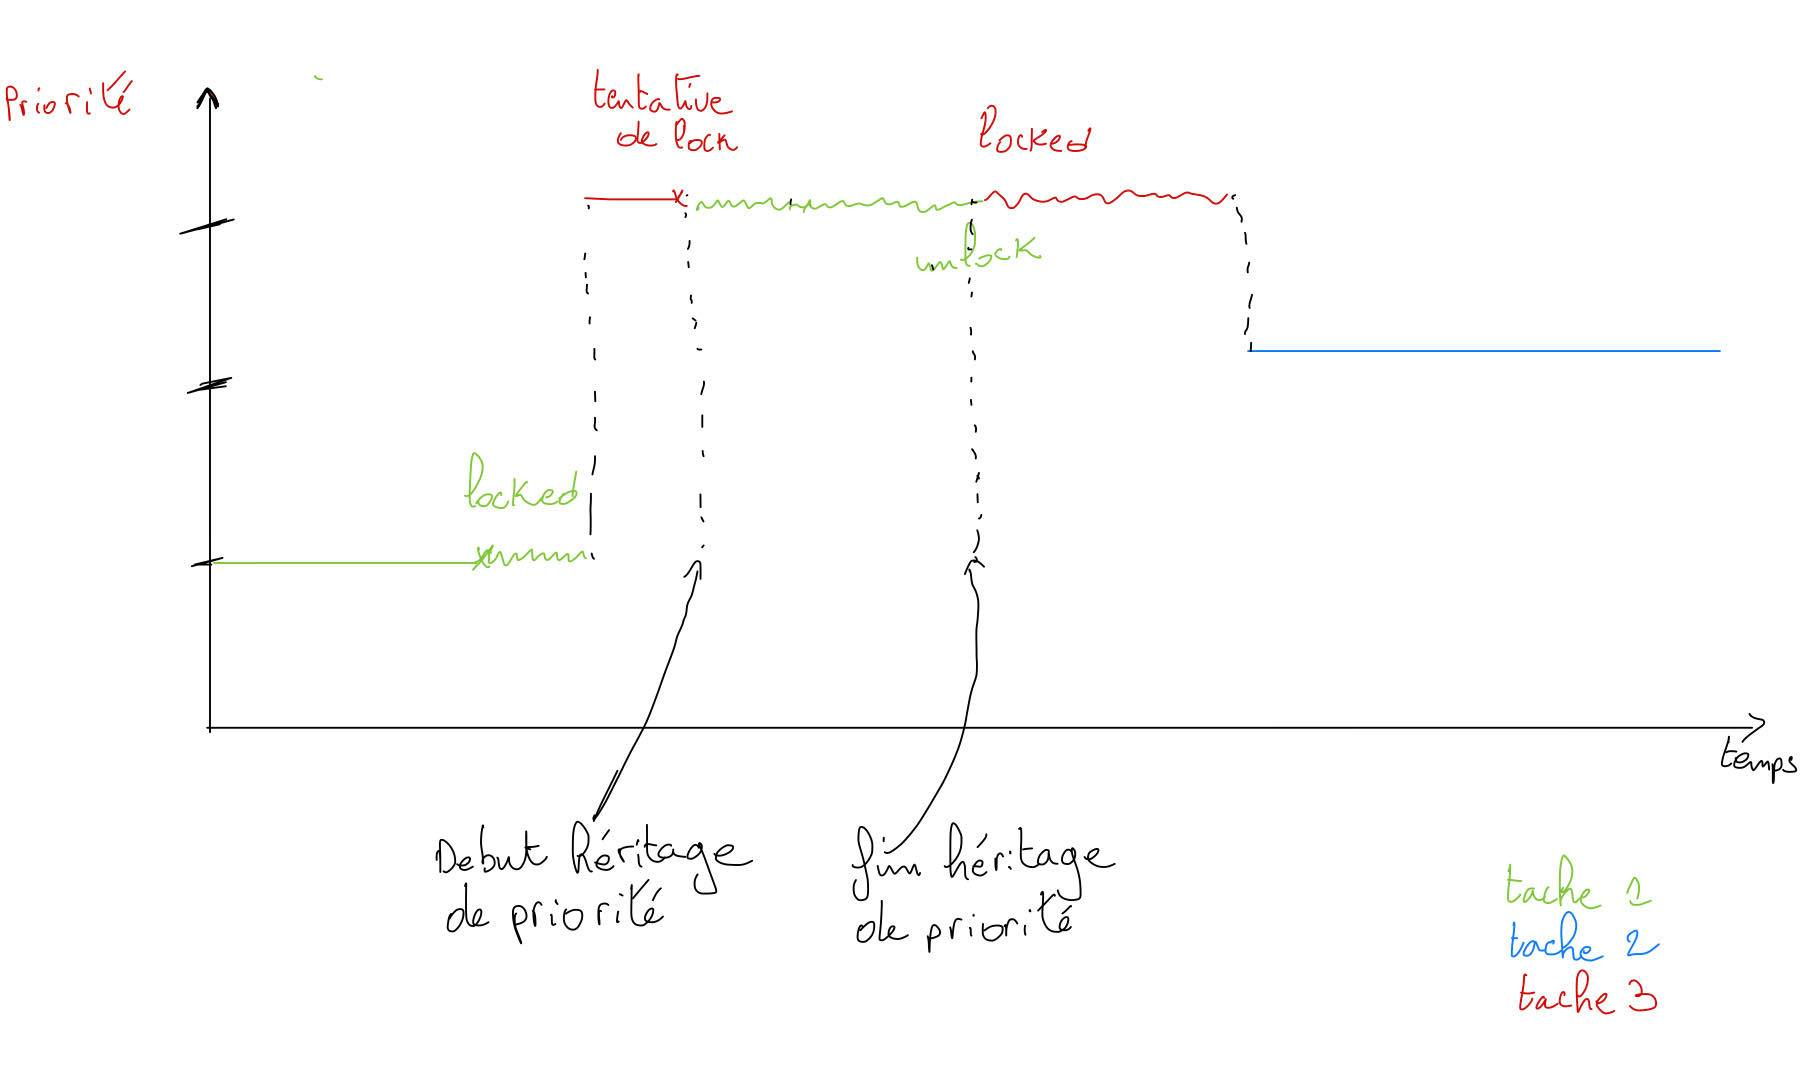
\includegraphics[scale=0.21]{include/with_inherit.jpg}
	\caption{Avancement des processus avec l'heritage de priorité}
	\label{fig:with_inherit}
\end{figure}

Le CFS est connu pour être un scheduler très équitable, en combinant ces deux techniques cela permet d'assurer une implémentation qui reste juste pour chaque tâche.